\documentclass{article}

\usepackage[utf8]{inputenc}
\usepackage{longtable}
\usepackage{adjustbox}
\usepackage{natbib}


\title{INDICES DE COLOMBIA}
\author{
        Nicolás Ramírez Pérez\\
        Facultad de Ingeniería\\
        Universidad de los Andes\\
        Bogotá,\underline{Colombia}\\
        \texttt{n.ramirez12@uniandes.edu.co}
}
\date{30 de Junio de 2018}

\usepackage{Sweave}
\begin{document}
\Sconcordance{concordance:ProyectoFInal.tex:ProyectoFInal.Rnw:%
1 18 1 1 0 15 1 1 2 4 1 1 8 2 1 1 7 14 0 1 3 1 1 1 8 1 3 4 1 1 10 13 0 %
1 2 2 1 1 8 1 3 5 1}

\maketitle


\begin{abstract}
Este es el proyecto final del curso dictado en la universidad de los Andes en la ciudad de Bogotá,Colombia. Este trabajo fue hecho bajo la filosofía de trabajo replicable.Este es el proyecto final del curso dictado en la universidad de los Andes en la ciudad de Bogotá,Colombia. Este trabajo fue hecho bajo la filosofía de trabajo replicable.Este es el proyecto final del curso dictado en la universidad de los Andes en la ciudad de Bogotá,Colombia. Este trabajo fue hecho bajo la filosofía de trabajo replicable.
\end{abstract}



\section*{Introducción}

Estos son los indices de Colombia, siguiendo la logica del paper realizado en la clase anterior. Estos son los indices de Colombia, siguiendo la logica del paper realizado en la clase anterior. Estos son los indices de Colombia, siguiendo la logica del paper realizado en la clase anterior. Estos son los indices de Colombia, siguiendo la logica del paper realizado en la clase anterior

Para comenzar veremos la sección \ref{univariada} en la página \pageref{univariada}.
\clearpage

\section{Exploración Univariada}\label{univariada}
En esta seccion se explorara cada indice que nos dara el profesor Jose Magallanes, bajo en codigo estadistico desarrollado por el.En esta seccion se explorara cada indice que nos dara el profesor Jose Magallanes, bajo en codigo estadistico desarrollado por el.En esta seccion se explorara cada indice que nos dara el profesor Jose Magallanes, bajo en codigo estadistico desarrollado por el.


Para conocer el comportamiento de las variables se preparo la Tabla \ref{stats}, donde se muestra los estadisticos de \emph{IDH}, \emph{Población Cabecera}  y \emph{Poblacion Resto}. Igualmente se muestra los histogramas correspondientes \ref{histog}

% Table created by stargazer v.5.2.2 by Marek Hlavac, Harvard University. E-mail: hlavac at fas.harvard.edu
% Date and time: jue., jul. 05, 2018 - 12:03:09 a. m.
\begin{table}[!htbp] \centering 
  \caption{Medidas estadisticas} 
  \label{stats} 
\begin{tabular}{@{\extracolsep{5pt}}lcccc} 
\\[-1.8ex]\hline 
\hline \\[-1.8ex] 
Statistic & \multicolumn{1}{c}{N} & \multicolumn{1}{c}{Min} & \multicolumn{1}{c}{Median} & \multicolumn{1}{c}{Max} \\ 
\hline \\[-1.8ex] 
IDH & 32 & 0.691 & 0.804 & 0.879 \\ 
Población.Cabecera & 32 & 13,090 & 717,197 & 10,070,801 \\ 
Población.Resto & 32 & 21,926 & 268,111.5 & 1,428,858 \\ 
\hline \\[-1.8ex] 
\end{tabular} 
\end{table} \begin{figure}[h]
\centering
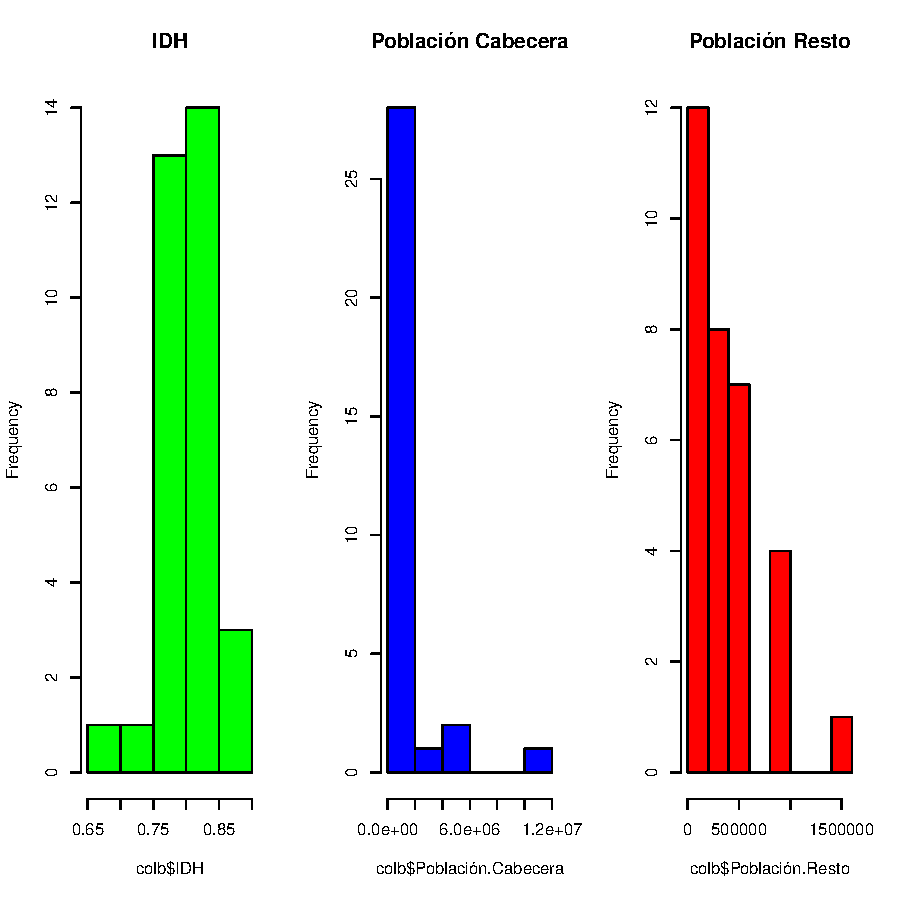
\includegraphics{ProyectoFInal-histogramas}
\caption{Histogramas variables de interes}
\label{histog}
\end{figure}

Debido a que existe sesgo en las poblaciones, seran transformados los datos con los cuales se realizo \ref{stats} (ver en la pag. \pageref{stats}) y se presentaran en la tabla \ref{stats1} y se presenta nuevamente los histogramas \ref{histog1}.
% Table created by stargazer v.5.2.2 by Marek Hlavac, Harvard University. E-mail: hlavac at fas.harvard.edu
% Date and time: jue., jul. 05, 2018 - 12:03:09 a. m.
\begin{table}[!htbp] \centering 
  \caption{Medidas estadisticas datos Transformados} 
  \label{stats1} 
\begin{tabular}{@{\extracolsep{5pt}}lcccc} 
\\[-1.8ex]\hline 
\hline \\[-1.8ex] 
Statistic & \multicolumn{1}{c}{N} & \multicolumn{1}{c}{Min} & \multicolumn{1}{c}{Median} & \multicolumn{1}{c}{Max} \\ 
\hline \\[-1.8ex] 
Cabecera.Transformada & 32 & 9.480 & 13.483 & 16.125 \\ 
Resto.Transformada & 32 & 9.995 & 12.499 & 14.172 \\ 
\hline \\[-1.8ex] 
\end{tabular} 
\end{table} 
\begin{figure}[h]
\centering
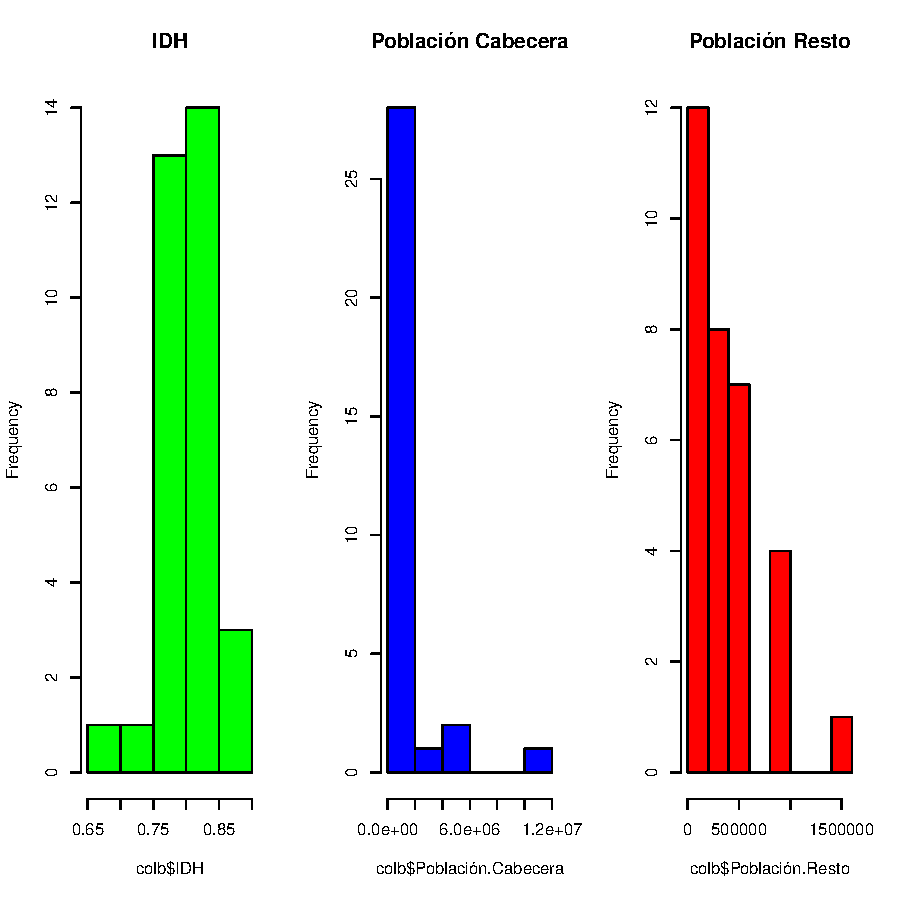
\includegraphics{ProyectoFInal-histogramas}
\caption{Histogramas variables de interes transformados}
\label{histog1}
\end{figure}
\clearpage
\section{Exploración Bivariada}\label{bivariada}
En este trabajo estamos interesados en el impacto de la poblacion en el el IDH, esto se puede obrservar en la tabla \ref{cor}. 
% Table created by stargazer v.5.2.2 by Marek Hlavac, Harvard University. E-mail: hlavac at fas.harvard.edu
% Date and time: jue., jul. 05, 2018 - 12:03:09 a. m.
\begin{table}[!htbp] \centering 
  \caption{Correlaciones} 
  \label{cor} 
\begin{tabular}{@{\extracolsep{5pt}} cc} 
\\[-1.8ex]\hline 
\hline \\[-1.8ex] 
Cabecera.Transformada & Resto.Transformada \\ 
\hline \\[-1.8ex] 
$0.487$ & $0.177$ \\ 
\hline \\[-1.8ex] 
\end{tabular} 
\end{table} 
De igual manera, nos intera la correlacion de las variable independientes. Esto se puede observar en la Tabla \ref{correind} y en la Grafica \ref{corre}

% Table created by stargazer v.5.2.2 by Marek Hlavac, Harvard University. E-mail: hlavac at fas.harvard.edu
% Date and time: jue., jul. 05, 2018 - 12:03:09 a. m.
\begin{table}[!htbp] \centering 
  \caption{Correlaciones} 
  \label{correind} 
\begin{tabular}{@{\extracolsep{5pt}} ccc} 
\\[-1.8ex]\hline 
\hline \\[-1.8ex] 
 & Cabecera.Transformada & Resto.Transformada \\ 
\hline \\[-1.8ex] 
Cabecera.Transformada & $1$ & $0.840$ \\ 
Resto.Transformada & $0.840$ & $1$ \\ 
\hline \\[-1.8ex] 
\end{tabular} 
\end{table} 
\begin{figure}[h]
\centering
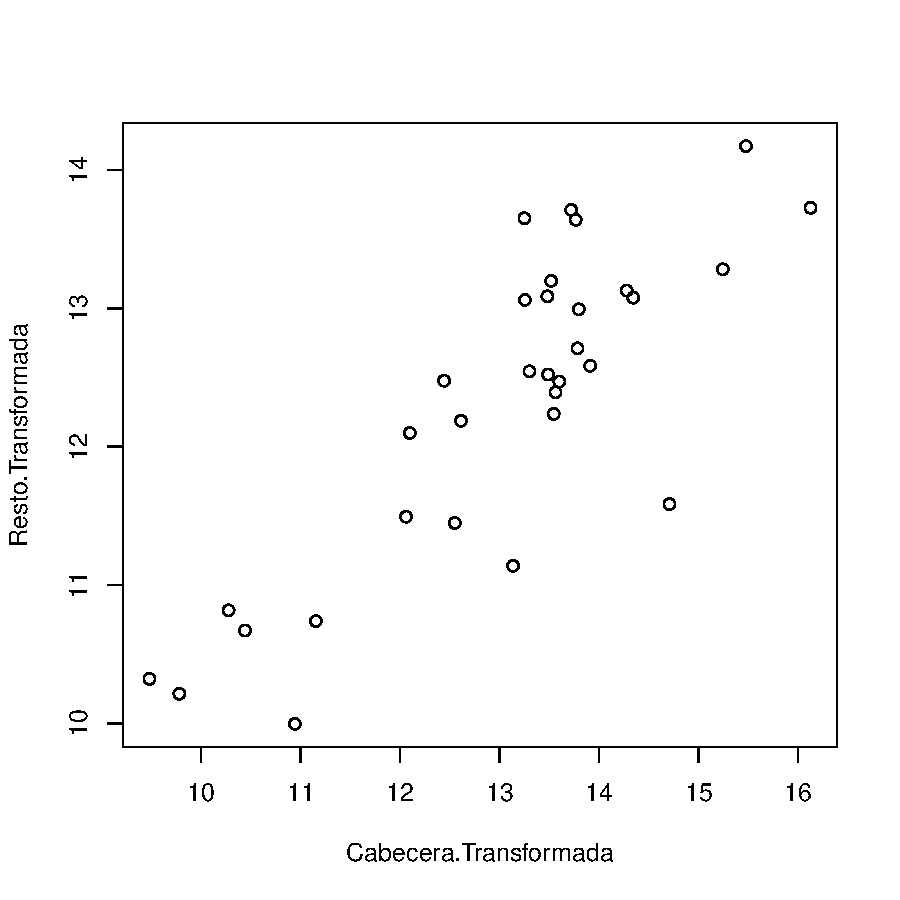
\includegraphics{ProyectoFInal-pcorre}
\caption{Correlaciones variables de interes transformados}
\label{corre}
\end{figure}
\clearpage

\section{Modelos de Regresión}\label{modelos}




En la tabla \ref{regA} se puede observar los resultados de la regresión lineal sin la variable Población resto. Por otra parte, se evidencia los resultados del modelo de regresión con la variable, anteriormente enunciada, en la tabla \ref{regB}
% Table created by stargazer v.5.2.2 by Marek Hlavac, Harvard University. E-mail: hlavac at fas.harvard.edu
% Date and time: jue., jul. 05, 2018 - 12:03:09 a. m.
\begin{table}[!htbp] \centering 
  \caption{Modelo de regresion sin población resto} 
  \label{regA} 
\begin{tabular}{@{\extracolsep{5pt}}lc} 
\\[-1.8ex]\hline 
\hline \\[-1.8ex] 
 & \multicolumn{1}{c}{\textit{Dependent variable:}} \\ 
\cline{2-2} 
\\[-1.8ex] & IDH \\ 
\hline \\[-1.8ex] 
 Cabecera.Transformada & 0.013$^{***}$ \\ 
  & (0.004) \\ 
  & \\ 
 Constant & 0.634$^{***}$ \\ 
  & (0.055) \\ 
  & \\ 
\hline \\[-1.8ex] 
Observations & 32 \\ 
R$^{2}$ & 0.238 \\ 
Adjusted R$^{2}$ & 0.212 \\ 
Residual Std. Error & 0.037 (df = 30) \\ 
F Statistic & 9.347$^{***}$ (df = 1; 30) \\ 
\hline 
\hline \\[-1.8ex] 
\textit{Note:}  & \multicolumn{1}{r}{$^{*}$p$<$0.1; $^{**}$p$<$0.05; $^{***}$p$<$0.01} \\ 
\end{tabular} 
\end{table} % Table created by stargazer v.5.2.2 by Marek Hlavac, Harvard University. E-mail: hlavac at fas.harvard.edu
% Date and time: jue., jul. 05, 2018 - 12:03:09 a. m.
\begin{table}[!htbp] \centering 
  \caption{Modelo de regresion con población resto} 
  \label{regB} 
\begin{tabular}{@{\extracolsep{5pt}}lc} 
\\[-1.8ex]\hline 
\hline \\[-1.8ex] 
 & \multicolumn{1}{c}{\textit{Dependent variable:}} \\ 
\cline{2-2} 
\\[-1.8ex] & IDH \\ 
\hline \\[-1.8ex] 
 Cabecera.Transformada & 0.013$^{***}$ \\ 
  & (0.004) \\ 
  & \\ 
 Constant & 0.634$^{***}$ \\ 
  & (0.055) \\ 
  & \\ 
\hline \\[-1.8ex] 
Observations & 32 \\ 
R$^{2}$ & 0.238 \\ 
Adjusted R$^{2}$ & 0.212 \\ 
Residual Std. Error & 0.037 (df = 30) \\ 
F Statistic & 9.347$^{***}$ (df = 1; 30) \\ 
\hline 
\hline \\[-1.8ex] 
\textit{Note:}  & \multicolumn{1}{r}{$^{*}$p$<$0.1; $^{**}$p$<$0.05; $^{***}$p$<$0.01} \\ 
\end{tabular} 
\end{table} \section{Exploración Espacial}\label{espacial}
Calculemos conglomerados de regiones, usando toda la información de las tres variables. Usaremos la tecnica de k-means propuesta por MacQueen \cite{macqueen_methods_nodate}



\begin{figure}[h]
\centering

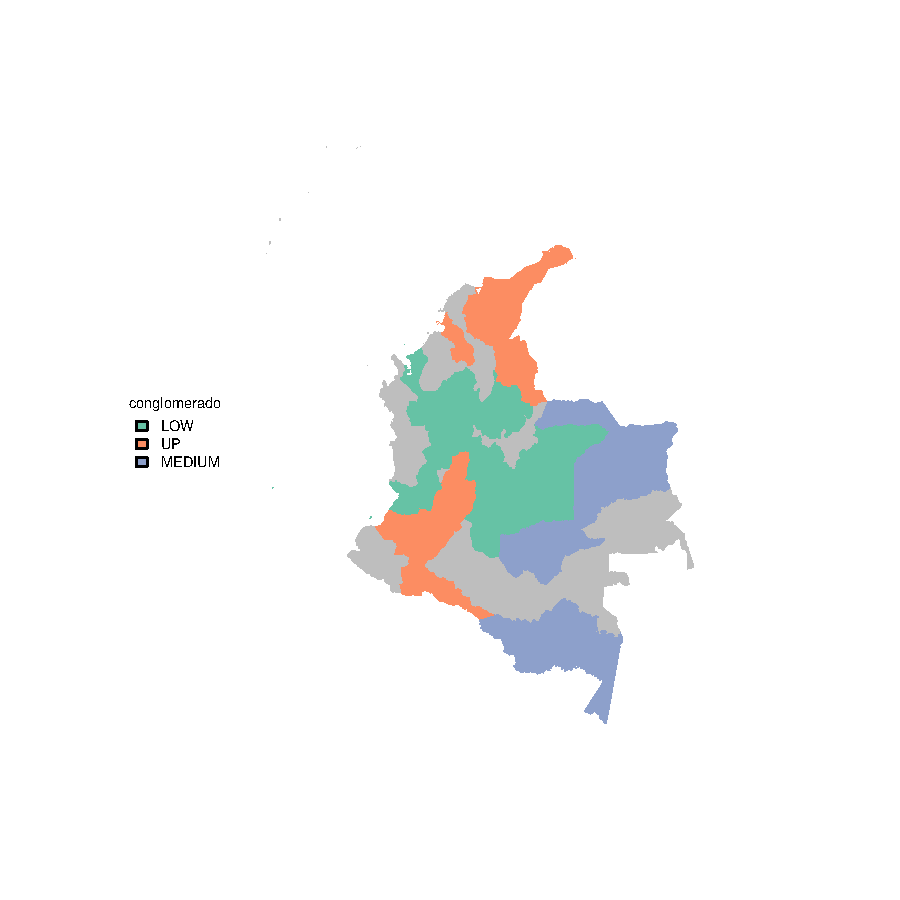
\includegraphics{ProyectoFInal-plotMap1}

\caption{Departamentos conglomerados segun sus indicadores}\label{clustmap}
\end{figure}


\bibliographystyle{abbrv}
\renewcommand{\refname}{Bibliografía}
\bibliography{proyecto}

\end{document}
